% ============================================================
% NERCCS 2026 — In-Person Attendee & Presenter Logistics
% ============================================================

\documentclass[11pt]{article}
\usepackage{kpfonts}
\usepackage[margin=1in]{geometry}
\usepackage[T1]{fontenc}
\usepackage{microtype}
\usepackage[hidelinks]{hyperref}
\usepackage{enumitem}
\usepackage{titlesec}
\usepackage{fancyhdr}
\usepackage{xcolor}
\usepackage{graphicx}
\pagestyle{fancy}
\fancyhf{}
\lhead{NERCCS 2026}
\rhead{In-Person Logistics}
\cfoot{\thepage}

\titleformat{\section}{\Large\bfseries}{}{0pt}{}[\vspace{-0.3em}\rule{\textwidth}{0.4pt}]
\titleformat{\subsection}{\large\bfseries}{}{0pt}{}

\setlist[itemize]{itemsep=0.3em, topsep=0.3em}

% ============================================================
\begin{document}

\begin{center}
    {\LARGE\bfseries NERCCS 2026 — In-Person Logistics}\\[0.5em]
    {\large Ninth Northeast Regional Conference on Complex Systems}\\[0.3em]
    {\normalsize March 11--13, 2026 \quad|\quad University of Rochester}\\[0.3em]
    {\normalsize Questions? \href{mailto:nerccs2026@gmail.com}{nerccs2026@gmail.com}}
\end{center}

\vspace{1em}

% ============================================================
\section{Venue}

\textbf{Robert B. Goergen Hall for Biomedical Engineering and Optics}\\
480 Intercampus Drive, Rochester, NY 14620\\[0.5em]

\begin{itemize}
    \item \textbf{Sloan Auditorium (Goergen 101)} --- Keynotes and main plenary sessions
    \item \textbf{Fantone Lecture Hall (Goergen 109)} --- Parallel sessions
    \item \textbf{Munnerlyn Atrium} --- Registration, coffee, breakfast, and lunch
\end{itemize}

% ============================================================
\section{Parking}

\subsection{Recommended Lot}

\begin{figure}[h]
	\centering
	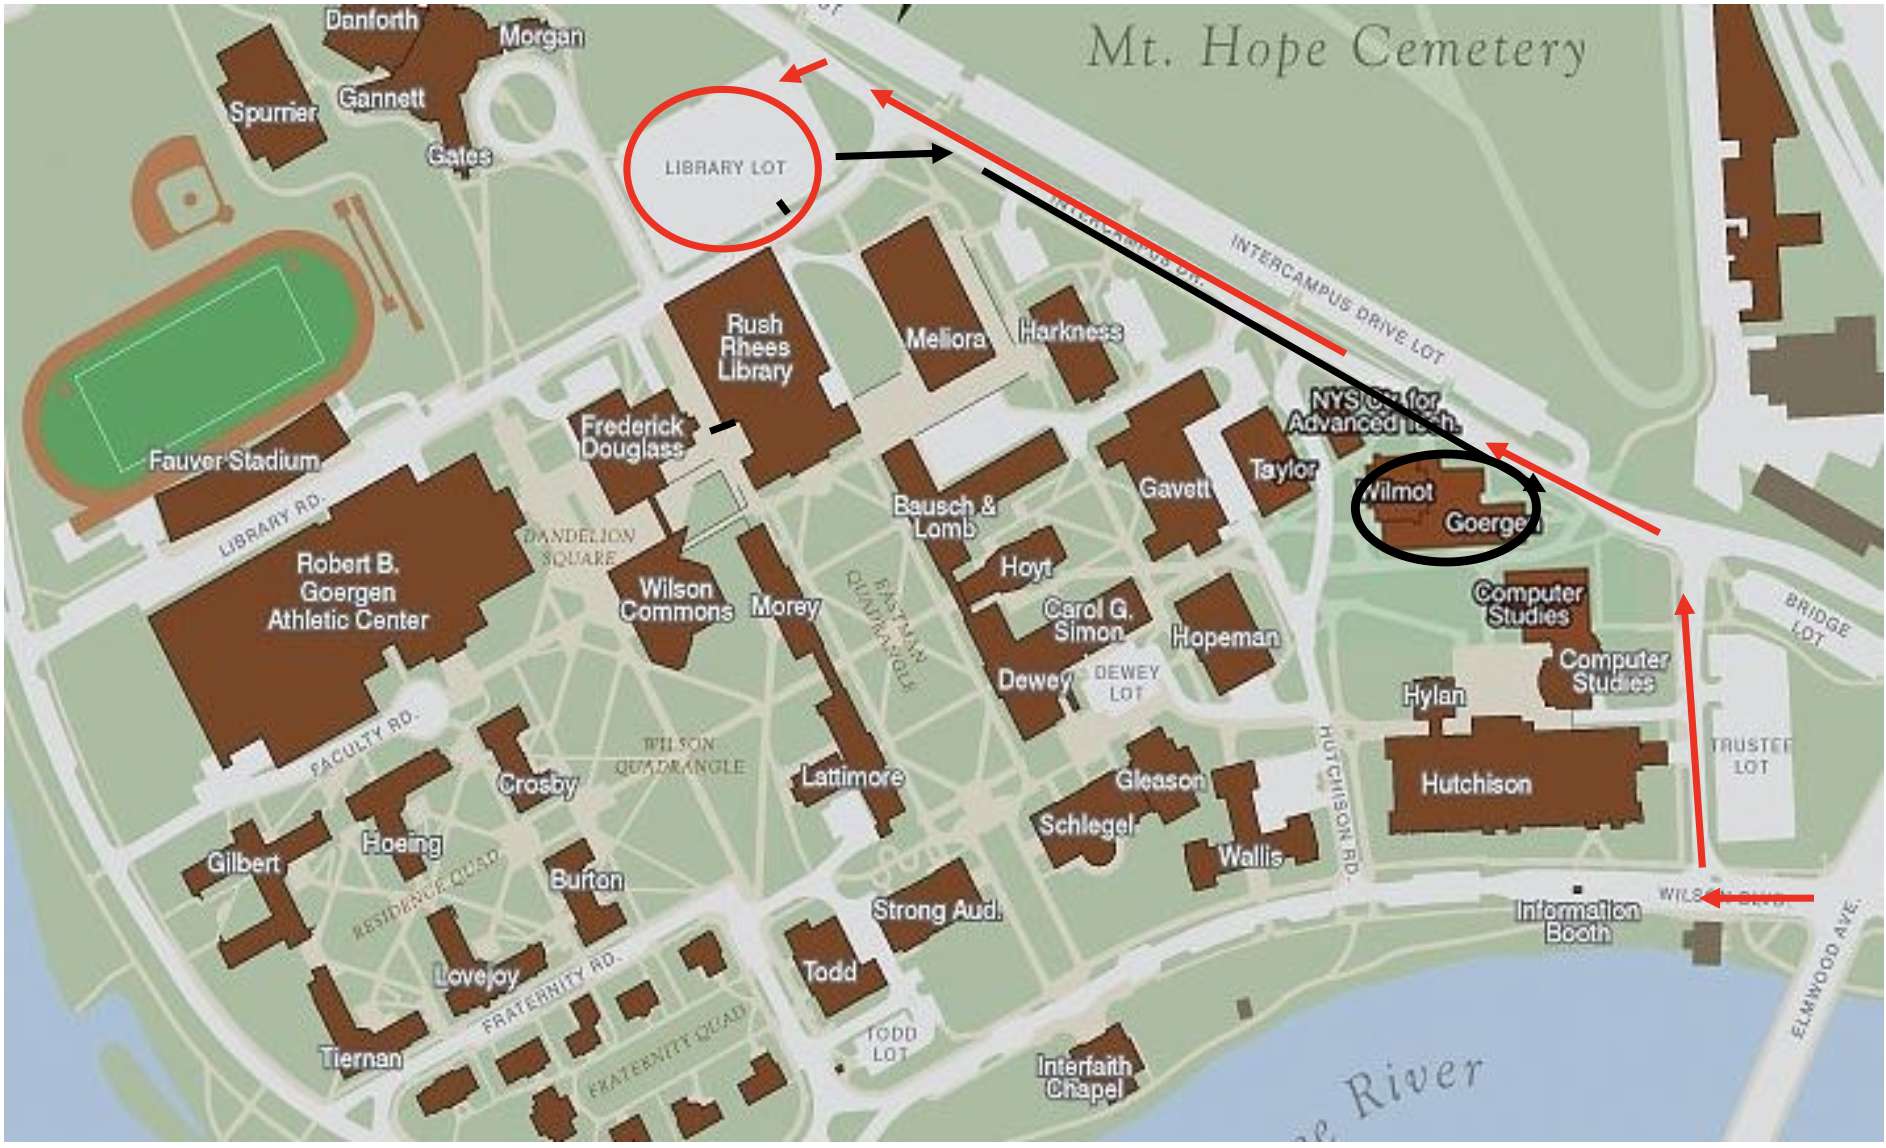
\includegraphics[width=\linewidth]{parkingMap}

\end{figure}

Red = Driving + Parking Directions

Black = Walking Directions


Once you enter the University of Rochester River Campus from Elmwood
Avenue, turn right on Trustee Road, then left on Intercampus Drive and follow the
road until you get to the Library Lot’s main entrance on your left.


If you are entering from the Ford Bridge/ Wilson Boulevard side, please go
straight on Wilson Boulevard, then turn left on Intercampus Drive, drive up the
hill and you will see the Library Lot’s entrance on your right.

At the gate, please use \fbox{\textbf{parking code 586944}.}


% ============================================================
\section{Getting There}

\subsection{By Car}
[PLACEHOLDER: Brief driving directions or note to use GPS address above.]

\subsection{By Public Transit}
Rochester RTS bus information: \href{https://www.myrts.com/}{myrts.com}\\
[PLACEHOLDER: Relevant route number(s) and stop nearest Goergen Hall.]

\subsection{From the Airport}
Rochester Douglas International Airport (ROC) is approximately [PLACEHOLDER: distance/time] from campus.\\
[PLACEHOLDER: Taxi/rideshare notes, shuttle info if any.]

% ============================================================
\section{Registration Check-In}

Registration and badge pickup will be in the \textbf{Munnerlyn Atrium} (Goergen Hall ground floor).\\[0.3em]
\textbf{Check-in hours:}
\begin{itemize}
    \item Wednesday, March 11: 12:00 pm -- 4:00 pm
    \item Thursday, March 12: 8:00 am -- 1:00 pm
    \item Friday, March 13: 8:00 am -- 11:00 am
\end{itemize}

% ============================================================
\section{Food \& Meals}

\begin{itemize}
    \item \textbf{Coffee/refreshments} will be provided each morning and at breaks in the Munnerlyn Atrium.
    \item \textbf{Buffet lunch} is provided on Thursday, March 12 (11:30 am -- 1:30 pm) in the Munnerlyn Atrium.
    \item Lunch is \textbf{not} provided on Wednesday or Friday; nearby dining options are listed below.
\end{itemize}

\subsection{Nearby Dining}
[PLACEHOLDER: List 3--5 nearby restaurants/cafes with approximate walking distance.]

% ============================================================
\section{Wi-Fi Access}

\textbf{Network:} [PLACEHOLDER: network name, e.g., ``URochester-Guest'']\\
\textbf{Password:} [PLACEHOLDER: password, or ``no password required'']\\
[PLACEHOLDER: Any login portal instructions.]

% ============================================================
\section{Accessibility}

[PLACEHOLDER: Elevator locations, accessible restroom locations, quiet space availability,
and any other accessibility accommodations. Contact info for accessibility needs.]

% ============================================================
\section{For Presenters}

\begin{itemize}
    \item \textbf{Talk slots are 20 minutes} (15 min talk + 5 min Q\&A).
    \item Please arrive at your session room \textbf{at least 10 minutes before the 
    session begins} to prepare the presentation.
    \item Please bring your own laptop (or a USB key with your slides prepared) 10 
    minutes before the parallel session begins and connect to the Zoom link.

\end{itemize}

\subsection{Zoom Meeting Links}

There are two simultaneous rooms during parallel sessions.
Check the program book to determine which room your talk or session of interest is 
in.

\subsubsection*{Room 1 — Sloan Auditorium (Goergen 101)}
\textit{Keynotes and parallel sessions are held here.}\\[0.5em]
\fbox{\href{https://urldefense.com/v3/__https://binghamton.zoom.us/j/94357348766?pwd=ge9FpadxB3UZEP22PRQobi5IFN5lf2.1__;!!CGUSO5OYRnA7CQ!dW3ugPLmcMfaZh66MWN5oPZY928T9HTfsPxpP_r4pJXh2xVGix5yc_bhmenhROG18LhWDL0_-GMfGC7YaUPKjFIVj9a7$}{\textbf{Zoom
			Link for Sloan Auditorium}}}\\

\subsubsection*{Room 2 — Fantone Lecture Hall (Goergen 109)}
\textit{Parallel sessions only; no keynotes in this room.}\\[0.5em]
\fbox{\href{https://urldefense.com/v3/__https://binghamton.zoom.us/j/98192108895?pwd=0glaVwEq8VG5LqY95xJENaFKXStSaG.1__;!!CGUSO5OYRnA7CQ!dW3ugPLmcMfaZh66MWN5oPZY928T9HTfsPxpP_r4pJXh2xVGix5yc_bhmenhROG18LhWDL0_-GMfGC7YaUPKjAkP6nLS$}{\textbf{Zoom
			link for Fantone Lecture Hall}}}\\

% ============================================================
\section{Emergency \& Safety Information}

\textbf{Emergency:} Call 911\\
\textbf{University of Rochester Campus Security:} [PLACEHOLDER: phone number]\\
\textbf{Nearest hospital/urgent care:} [PLACEHOLDER: name and address]\\[0.3em]
[PLACEHOLDER: Location of AED units and first aid kits in Goergen Hall.]

% ============================================================
\section{Contact}

Conference email: \href{mailto:nerccs2026@gmail.com}{nerccs2026@gmail.com}\\[0.3em]
\textbf{On-site contacts (day-of):}\\
[PLACEHOLDER: Name and cell number of logistics contact(s).]

\end{document}
